\chapter{Contexte}     % numéroté
\label{chap:background}                   % étiquette pour renvois (à compléter!)

En premier lieu, nous allons commencer par faire une brève revue des différentes catégories  de méthodes de détection d'anomalies et de leur fonctionnement respectif. Ensuite, nous allons faire un résumé de la théorie des autoencodeurs et comment ceux-ci sont pertinents dans un contexte de détection d'anomalies. Ensuite, nous allons décrire plus en détails un type particulier d'autoencodeur utilisé dans cette étude, soit l'autoencodeur variationnel. Finalement, nous allons couvrir quelques notions de base quant aux tests d'hypothèses, un cadre statistique classique pour prendre des décisions.

\section{Les méthodes de détection d'anomalies}

Tout d'abord, il est pertinent de commencer par mentionner que toutes les méthodes de détection d'anomalies fonctionnent fondamentalement de la même manière. En effet, ces algorithmes sont en mesure de faire l'apprentissage d'un jeu de données et de stocker cette information dans un modèle d'apprentissage. En sachant ce qui est normal, il est donc également possible d'utiliser ce modèle pour évaluer ce qui est anormal en identifiant ce qui dévie de cette normalité. Le choix du modèle est cruciale, car si celui-ci ne s'ajuste pas bien aux données, il pourrait nous induire en erreur sur l'anormalité d'une observation \citep{10.5555/3086742}. 

Pour démontrer l'importance du choix de modèle, prenons un exemple simpliste et fréquemment utilisé en pratique, soit sur la moyenne d'une loi normale à variance connue, souvent appelé le test $Z$. Dans ce test statistique, qui peut être utilisé pour de la détection d'anomalies, l'hypothèse nulle est que les données suivent une loi normale. Prenons par exemple des observations à $1$ dimension $X_1, ..., X_N$ avec de moyenne $\mu$ et d'écart-type $\sigma$. La valeur $Z$ pour une observation $X_i$ est donnée par :

\begin{gather}
Z_i = \frac{|X_i-\mu|}{\sigma}.
\end{gather}

Cette valeur $Z$ nous donne en fait le nombre d'écarts-types dont une observation dévie de la moyenne. On peut généralement penser que si une observation dévie beaucoup de la moyenne, ça peut être un indicateur important d'anomalie. Dans ce cas-ci, on utilise généralement la règle du pouce $Z_i \ge 3$ comme indicateur d'anomalie. En d'autres mots, une observation est improbable, ou potentiellement "anormale", si elle se situe à plus ou moins 3 écarts-types de la moyenne. Ce modèle de détection d'anomalie s'applique bien dans le cas où nos observations proviennent réellement d'une loi normale. Dans la figure \ref{fig:Ztest_a}, on peut voir 5000 simulations d'une loi normale de moyenne nulle et d'écart-type égale à 2. On peut voir que notre règle du pouce, ou notre modèle, fonctionne relativement bien puisque les valeurs se situant à l'extérieur de l'intervalle $[-6, 6]$ ont tous une fréquence relative très faible. De la même manière, les valeurs se situant à l'intérieur de l'intervalle $[-6, 6]$ ont des fréquence relative acceptable ($\ge 0.5\%$). Cela nous laisse croire que la détection d'anomalies est adéquate. Dans une autre situation où les données ne proviennent pas d'une loi normale, notre règle du pouce, ou notre modèle, peut être moins adéquat. Supposons que nos données proviennent plutôt d'une loi à queue lourde, comme la loi standard Cauchy. En simulant $5000$ observations de cette loi, nous obtenons une moyenne empirique de $-1.6$ et un écart-type empirique de $160.2$. C'est donc dire que l'intervalle défini avec le modèle précédent serait de $[-482.2, 479]$. On peut voir à la figure \ref{fig:Ztest_b} que plusieurs observations ne sont pas considérées comme des anomalies selon ce modèle, alors que leur fréquence relative est pourtant très faible (par exemple inférieure à $0.5\%$). 

\begin{figure}[htb]
	\centering
	\begin{subfigure}{6cm}
		\centering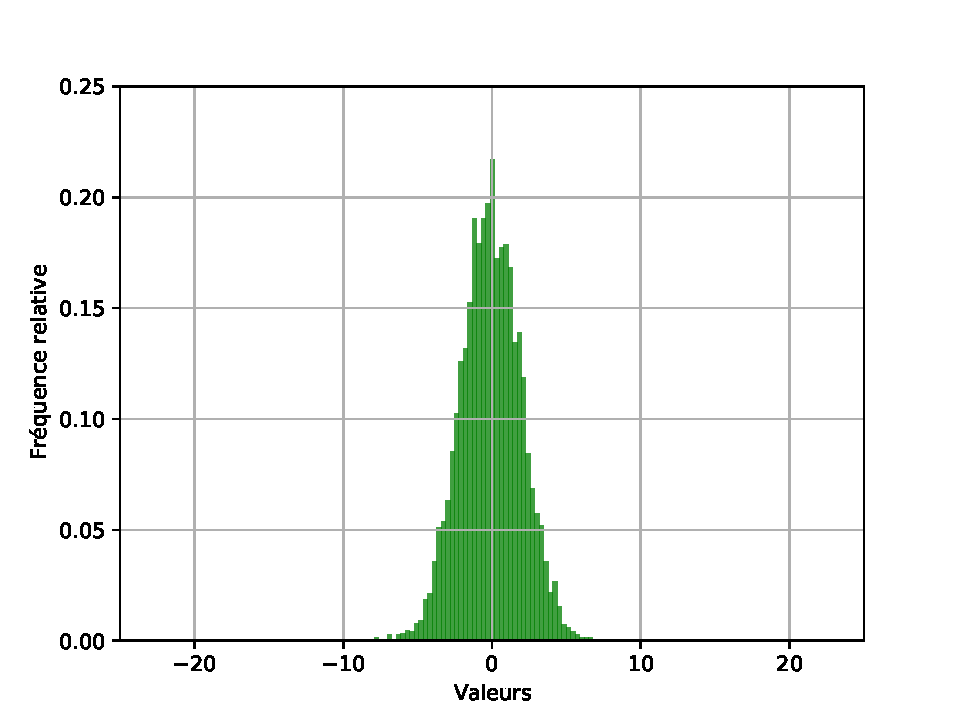
\includegraphics[width=6cm]{images/histogram-normal-ztest}
		\caption{Distribution normale}
		\label{fig:Ztest_a}
	\end{subfigure}
	\begin{subfigure}{6cm}
		\centering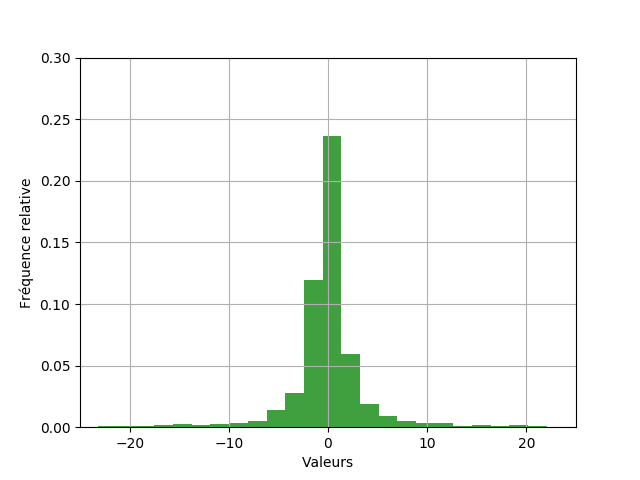
\includegraphics[width=6cm]{images/histogram-cauchy-ztest}
		\caption{Distribution standard Cauchy}
		\label{fig:Ztest_b}
	\end{subfigure}
	\caption{Distribution de 5000 simulations d'une loi normale et d'une loi standard Cauchy}
	\label{fig:ZTest}
\end{figure}

L'exemple du test $Z$ illustre simplement le fait que le choix du modèle aura un impact important dans la détection d'anomalies. Au final, la pertinence du modèle choisi sera étroitement lié à la nature des données. Il existe plusieurs catégories d'algorithmes de détection d'anomalies. Dans \cite{10.5555/3086742}, 4 de ces approches nous apparaissent comme particulièrement intéressantes à survoler.

\subsection{Analyse des valeurs extrêmes}

La détection d'anomalies via l'analyse des valeurs extrêmes est probablement une des approches les plus simples. Dans un cas à une seule dimension, les anomalies sont définies comme les valeurs très grandes ou très faibles par rapport à la majorité des autres valeurs. On s'intéresse donc à la queue d'une distribution, comme dans l'exemple avec le test $Z$ présenté plus tôt. Cette approche vient légèrement à l'encontre de la définition d'une anomalie présentée plus tôt où l'accent est plutôt mis sur le fait qu'une anomalie diffère de la majorité des données. Cette dernière définition fait davantage référence à une notion de probabilité.

Bien que l'analyse des valeurs extrêmes ne soit pas la méthode la plus utilisée en pratique pour identifier des anomalies, elle fait souvent partie intégrante de plusieurs autres méthodes. En effet, l'analyse de valeurs extrêmes est souvent utilisée comme étape finale de plusieurs autres algorithmes. C'est d'ailleurs ce qui permet généralement de déterminer ce qui dévie d'une certaine normalité, via une valeur unidimensionnelle comme un score d'anomalie ou une distance.


\subsection{Les modèles probabilistes}

L'élément clé des approches basées sur des modèles probabilistes  est qu'on fait une hypothèse sur la distribution des données. Ensuite, on ajuste le modèle statistique correspondant à cette hypothèse sur les données en faisant l'apprentissage des paramètres du modèle. Un exemple classique pourrait être d'ajuster un mélange de $k$ lois normales. Avec ce modèle, on fait l'hypothèse que chaque observation provient d'un des $k$ groupes de la loi mélange. On peut faire l'apprentissage des paramètres du modèle avec l'algorithme \textit{expectation-maximization (EM)}. Par la suite, on peut évaluer l'anormalité d'une observation en se basant sur la probabilité de cette instance selon notre modèle ajusté. Ce type d'approche a l'avantage de pouvoir s'appliquer assez facilement à plusieurs types de données. Par contre, le désavantage est que l'on doit faire une hypothèse quant à la distribution des données, qui peut parfois être inadéquate. Certains jeux de données peuvent difficilement être représenté par une distribution connue, ce qui peut mener à un mauvais ajustement du modèle et ainsi tirer de mauvaises conclusions quant à la nature d'une observation.

\subsection{Les modèles linéaires et non-linéaires} \label{soussec:linear}

Ce type d'approche est basé sur l'apprentissage d'un espace à plus petites dimensions via un modèle linéaire ou non-linéaire. Un exemple classique est l'utilisation d'une régression linéaire. Par exemple, dans un cas d'une régression linéaire à 2 variables explicatives, l'apprentissage d'une variable réponse $y_i$ est donnée par l'équation \ref{eq_reg}. Dans ce cas-ci, on utilise généralement la méthode des moindres carrés pour trouver les paramètres optimaux du modèle, soit les paramètres $\beta_0$, $\beta_1$ et $\beta_2$.

\begin{gather}  \label{eq_reg}
y_i = \beta_0 + \beta_{1} x_{1,i} + \beta_2 x_{2,i} + \epsilon_{i} \qquad \forall i \in {1,...,N}
\end{gather}

Les estimations de ces paramètres, soit $\hat{\beta_0}$, $\hat{\beta_1}$ et $\hat{\beta_2}$, nous permettent d'estimer la variable réponse $\hat{y_i}$: 

\begin{gather}  \label{eq_reghat}
\hat{y_i} = \hat{\beta_0} + \hat{\beta_{1}} x_{1,i} + \hat{\beta_2} x_{2,i} \qquad \forall i \in {1,...,N}
\end{gather}

On peut ensuite utiliser l'erreur de prédiction comme indicateur d'anomalie. Cette erreur de prédiction, défini comme $\hat{y_i} - y_i$, est également appelée erreur de reconstruction. La prémisse de base est que si le modèle est en mesure de bien ajuster les données, les observations normales devraient être bien reconstruites par le modèle. À l'inverse, les observations anormales devraient être mal reconstruites par le modèle.  On peut d'ailleurs ce servir encore une fois de l'analyse des cas extrêmes pour reconnaître les erreurs les plus importantes, et par le fait même, les anomalies.
 
Un autre exemple classique dans cette catégorie d'approches est l'utilisation d'une analyse en composante principale (ACP). Dans ce cas-ci, nous n'avons pas de variable réponse $y_i$ sur laquelle calculer une erreur de reconstruction. L'erreur de reconstruction sera donc basée sur la capacité de reconstruire l'entrée $x_i$. Cette technique de réduction de dimensionnalité permet de transformer les données vers un espace où les variables sont décorrélées et où l'utilisation d'un sous-ensemble de ces variables latentes peut être suffisant pour expliquer une bonne partie de la variabilité des données originales. La transformation permettant d'obtenir un espace latent à $k$ dimensions est donnée par l'équation \ref{eq_pca1}.
 
 \begin{gather}  \label{eq_pca1}
 Z = XV
 \end{gather}
 
Dans l'équation \ref{eq_pca1}, $X$ est une matrice $n \times p$ représentant les données initiales et où le vecteur de moyennes $\boldsymbol{\mu}$, calculé sur chaque colonne, a été soustrait à la matrice originale. $X$ est donc la matrice centrée des données initiales. $V$ représente une matrice $p \times k$, où $k < p$, de  vecteurs propres correspondant aux valeurs propres les plus élevées de la matrice de corrélation $\Sigma$. La valeur $k$ signifie qu'on conserve seulement $k$ variables latentes, ou également appelées composantes principales. La reconstruction de cet espace latent à $k$ dimensions peut ensuite être retrouvé par l'équation \ref{eq_pca2}. 
 
  \begin{gather}  \label{eq_pca2}
 \hat{X} = ZV^\top + \boldsymbol{\mu}
 \end{gather}
 
La projection de cet espace latent vers l'espace original défini par l'équation \ref{eq_pca2} permet d'obtenir une erreur de reconstruction. Celle-ci est peut être obtenue par une fonction appliquée entre $\hat{X}$ et $X$. Par exemple, on pourrait prendre la distance quadratique entre chaque instances de $\hat{X}$ et $X$ et ainsi obtenir $n$ erreurs de reconstruction. Cette erreur de reconstruction peut être utilisée pour trouver les observations qui dévie de la normalité du modèle de la même manière qu'avec une régression linéaire.
  
Cette catégorie d'approches de détection d'anomalies a le potentiel de mieux s'adapter à des données où il n'y a pas de distribution connue. La régression linéaire est un exemple de modèle linéaire, mais on pourrait également utiliser un modèle plus complexe qui permet de capture des non-linéarités. Par exemple, il est possible d'utiliser des réseaux de neurones pour faire l'apprentissage des données vers un espace à plus basse dimension. Le désavantage avec de telles approches est qu'on peut perdre la notion d'interpretabilité. Dans certains exemples d'applications, il peut être intéressant de savoir quelles raisons expliquent la présence d'une anomalie dans les données.

\subsection{Les méthodes basées sur les distances}

Cette catégorie de méthodes de détection d'anomalie est basée sur l'idée de trouver les observations qui sont isolées de la majorité des autres observations. Cela est généralement quantifié par des mesures de distances ou de dissimilarités. Parmi ces méthodes, on peut retrouver 3 sous-catégories fréquemment utilisées en pratique: les regroupements (\textit{clustering}), les méthodes de densité et les méthodes des plus proches voisin.

Dans le cas des regroupements et des méthodes de densité, l'objectif est de trouver des zones de l'espace qui caractérisent le jeu de données. Les anomalies sont généralement identifiées en considérant les observations qui ne font pas parties de ces zones. Dans le cas spécifique des regroupements, on fait un séparation de l'espace qui est basée sur les observations elles-mêmes. Si on prend comme exemple l'algorithme de regroupement $k$-moyennes, on peut évaluer le score d'anomalie d'une observation en prenant la distance minimale d'un centroïde trouvé pendant l'ajustement du modèle.

Dans les méthodes de densité, plutôt que séparer l'espace par l'entremise d'observations, on sépare directement des zones de cette espace. Ensuite, on évalue la densité des observations dans une zone selon le nombre d'observations dans cette même zone. Le fait de séparer l'espace des données nous permet de mieux quantifier la densité d'un point, peu importe son emplacement dans l'espace. Un exemple simple serait d'utiliser la méthode de l'histogramme afin de compartimenter l'espace en plusieurs sous-espaces et ensuite évaluer la densité d'une région par le nombre d'observations s'y retrouvant. Ce genre d'approche a généralement l'avantage d'être interprétable, car on peut savoir exactement pourquoi une observation fait partie d'un sous-ensemble ayant une faible densité. Prenons un exemple simple à seulement 2 dimensions où on retrouve le poids et la grandeur d'une personne. En séparant l'espace en différentes régions, on réalise que seulement très peu de personne ont un poids inférieur à 45 kg et une grandeur supérieur à 1.80 m. Ainsi, on peut facilement expliquer pourquoi une personne de 39 kg et de 1.85 m est considérée comme une anomalie. 
 
 Finalement, les méthodes basées sur les plus proches voisins permettent de définir un score d'anomalie qui dépend de la distance entre une observation et ses $k$ plus proches voisins. Plus cette distance est grande, plus on peut penser que la donnée est isolée du reste des autres observations. Encore une fois, on peut avoir recours à l'analyse des cas extrêmes pour évaluer à partir de quelle distance on peut considérer une donnée comme une anomalie.


\section{Les autoencodeurs}

Maintenant que nous avons couvert certaines notions de base par rapport à différentes approches de détection d'anomalie, nous allons couvrir la théorie de base derrière le fonctionnement des autoencodeurs. Comme mentionné dans la section \ref{soussec:linear}, certaines approches de modélisation plus complexes, comme les autoencodeurs, peuvent être utilisées pour faire l'apprentissage d'un jeu de données. 

Les premiers travaux se rapprochant de l'autoencodeur connu aujourd'hui remontent aux années 1980 \citep{Rumelhart-1986}. Dans ses travaux, le principe était d'apprendre une représentation cachée en utilisant l'entrée comme variable réponse. Avec la montée en popularité des réseaux de neurones au début des années 2000, une nouvelle génération d'autoencodeurs ont vu le jour. Ces autoencodeurs avaient désormais plusieurs couches cachées superposées \citep{HintonSalakhutdinov2006b}, permettant ainsi de faire l'apprentissage de données plus complexes comme des images. Un autoencodeur est un réseau de neurones qui a comme objectif d'apprendre une représentation intermédiaire et efficiente d'une entrée de manière non-supervisée \citep{Goodfellow-et-al-2016}. Pour réaliser cette objectif, l'autoencodeur se décompose en 2 composantes: un encodeur et un décodeur. L'encodeur reçoit en entrée $x$ et convertit celui-ci vers une représentation latente $z$. Le décodeur prend en entrée cette représentation latente $z$ et la décode pour ainsi retrouver le plus possible l'entrée initiale $x$. Cette structure de base est illustrée dans la figure \ref{fig:basicAE}. Historiquement, les autoencodeurs étaient vus comme une méthode de réduction de dimensionnalité, mais désormais ceux-ci ont davantage d'applications dû au fait qu'il peuvent apprendre des variables latentes riches en informations. On peut citer des applications en vision numérique pour retrouver le contenu d'une image \citep{conf/esann/KrizhevskyH11} ou même en traitement de la langue naturelle pour interpréter un discours oral \citep{inproceedings}. \newline

\begin{figure}[h]
	\centering
	\begin{tikzpicture}[shorten >=1pt,draw=black!50, node distance=\layersep, square/.style={regular polygon,regular polygon sides=4}]
	\tikzstyle{every pin edge}=[<-,shorten <=1pt]
	\tikzstyle{neuron}=[square,fill=black!25,minimum size=17pt,inner sep=0pt]
	\tikzstyle{input neuron}=[neuron, fill=green!50];
	\tikzstyle{output neuron}=[neuron, fill=red!50];
	\tikzstyle{hidden neuron1}=[neuron, fill=blue!50];
	\tikzstyle{hidden neuron2}=[neuron, fill=blue!50];
	\tikzstyle{hidden rep}=[neuron, fill=yellow!50];
	\tikzstyle{annot} = [text width=4em, text centered]
	
	% Draw the input layer nodes
	\foreach \name / \y in {1,...,4}
	% This is the same as writing \foreach \name / \y in {1/1,2/2,3/3,4/4}
	\node[input neuron] (I-\name) at (0,-\y) {};
	
	% Draw the hidden layer nodes n.1
	\foreach \name / \y in {1,...,2}
	\path[yshift=-1cm]
	node[hidden neuron1] (H1-\name) at (\layersep,-\y cm) {};
	
	% Draw the encoded representation
	\foreach \name / \y in {1,...,1}
	\path[yshift=-1.5cm]
	node[hidden rep] (R-\name) at (2 * \layersep,-\y cm) {};
	
	% Draw the hidden layer nodes n.2
	\foreach \name / \y in {1,...,2}
	\path[yshift=-1cm]
	node[hidden neuron1] (H2-\name) at (3 * \layersep,-\y cm) {};
	
	% Draw the output layer
	\foreach \name / \y in {1,...,4}
	% This is the same as writing \foreach \name / \y in {1/1,2/2,3/3,4/4}
	\node[output neuron] (O-\name) at (4 * \layersep,-\y cm) {};
	
	% Connect input
	\foreach \source in {1,...,4}
	\foreach \dest in {1,...,2}
	\path (I-\source) edge (H1-\dest);
	
	% Connect representation
	\foreach \source in {1,...,2}
	\foreach \dest in {1,...,1}
	\path (H1-\source) edge (R-\dest);
	
	\foreach \source in {1,...,1}
	\foreach \dest in {1,...,2}
	\path (R-\source) edge (H2-\dest);
	
	% Connect outputs
	\foreach \source in {1,...,2}
	\foreach \dest in {1,...,4}
	\path (H2-\source) edge (O-\dest);
	
	% Annotate the layers
	\node[annot,above of=I-1, node distance=1cm] (hl) {Couche d'entrée};
	\node[annot,above of=R-1, node distance=2.5cm][text width=8em] (hl) {Représentation \\ latente ($z$)};
	\node[annot,above of=O-1, node distance=1cm] (hl) {Couche de sortie};
	
	\draw [decorate,decoration={brace,mirror,amplitude=15pt},xshift=-4pt,yshift=-2cm]
	(0,-2.5) -- (4,-2.5) node [black,midway,yshift=-3em] 
	{\footnotesize encodeur: $q_{\theta}(x)$};
	\draw [decorate,decoration={brace,mirror,amplitude=15pt},xshift=4pt,yshift=-2cm]
	(4,-2.5) -- (8,-2.5) node [black,midway,yshift=-3em] 
	{\footnotesize décodeur: $p_{\phi}(z)$};
	
	\end{tikzpicture}
	\caption{Exemple illustrant la structure de base d'un autoencodeur. Dans le cas ci-dessus, on pourrait interpréter le schéma comme un réseau pleinement connecté où les blocs pourraient représentés les neurones et les liens seraient les poids, ou les paramètres du réseau. Le concept s'applique également à une architecture de réseau à convolutions, où les paramètres appris sont les filtres de convolutions.}
	\label{fig:basicAE}
\end{figure}

L'intuition derrière les autoencodeurs est essentiellement de reconstruire une entrée $x$ en passant par 2  fonctions (l'encodeur et le décodeur) apprises par le modèle. Ces deux fonctions vont permettre d'obtenir une sortie $\hat{x}$, donnée par l'équation:

\begin{gather} \label{eq:output}
	\hat{x} = p_\phi{\{q_\theta(x)\}}
\end{gather}

 Ainsi, ce genre de méthode n'a pas besoin d'une étiquette $y$, car son objectif est basé sur $x$ directement. C'est d'ailleurs pour cela qu'on parle d'une approche d'apprentissage non-supervisée. L'apprentissage des paramètres est fait en grande partie en minimisant l'erreur de reconstruction. La perte peut donc être définie par une fonction de la forme :

\begin{gather}  \label{eq:loss}
L(x, \hat{x}) = L(x, p_\phi{\{q_\theta(x)\}})
\end{gather}


\noindent où $q_{\theta}(\cdot)$ est l'encodeur et $p_{\phi}(\cdot)$ est le décodeur. L'optimisation de cette fonction de perte est faite par descente du gradient. En d'autres mots, les paramètres $\theta$ de l'encodeur et $\phi$ du décodeur sont optimisés graduellement en prenant la dérivée de la fonction de perte par rapport aux différents paramètres de ces deux composantes:


\begin{equation} \label{optim}
\Theta^{'} \leftarrow \Theta-\epsilon*\frac{\partial L}{\partial\Theta}
\end{equation}

\noindent où $\epsilon$ est un taux d'apprentissage qui permet de moduler la vitesse d'apprentissage et $\Theta = \{\theta, \phi\}$ comprend les paramètres de l'encodeur et du décodeur. $\Theta^{'}$ correspond aux valeurs des paramètres après avoir appliqué la correction d'une itération.

Illustrons l'apprentissage d'un autoencodeur de base avec un exemple simpliste. Supposons que nous avons en entrée un jeu de données $X$ avec $p=2$ variables et $n=10$ observations. Nous voulons encoder ces 2 variables dans une variable latente unidimensionnelle avec un autoencodeur à une seule couche cachée. Au total, notre autoencodeur possède 3 couches, soit une couche d'entrée, une couche cachée et une couche de sortie. Nous choisissons également une fonction d'activation sigmoïde pour notre couche cachée et une fonction d'activation linéaire pour notre couche de sortie. Les fonctions d'activation sont des transformations appliquées aux valeurs des neurones de notre réseau, ce qui permettra entres autres d'avoir un modèle non-linéaire, dans le cas de fonctions d'activation non-linéaires. L'architecture du réseau est définie dans la figure \ref{fig:toyAE}.

\begin{figure}[htb]
	\centering
	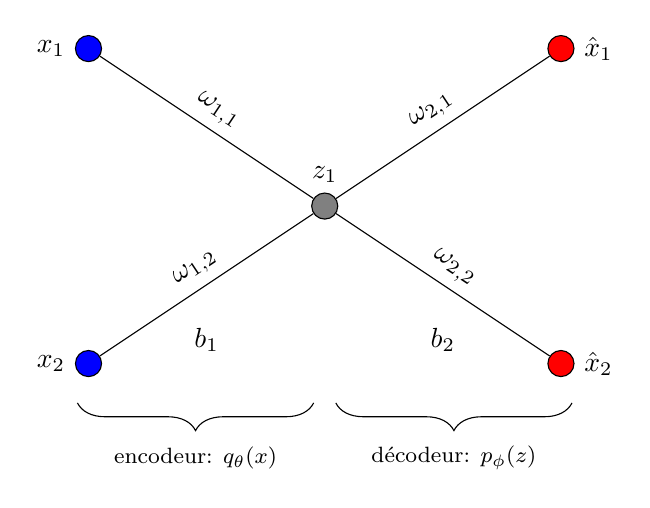
\begin{tikzpicture}
	[   cnode/.style={draw=black,fill=#1,minimum width=3mm,circle},
	]
	\node[cnode=blue,label=180:$x_{1}$] (x-1) at (0,2) {};
	\node[cnode=blue,label=180:$x_{2}$] (x-2) at (0,-2) {};
	\node[cnode=gray,label=90:$z_{1}$] (z) at (3,0) {};
	\node[cnode=red,label=0:$\hat{x}_{1}$] (x_chap-1) at (6,2) {};
	\node[cnode=red,label=0:$\hat{x}_{2}$] (x_chap-2) at (6,-2) {};
	
	\foreach \x in {1,2}
	{   \draw (x-\x) -- node[above,sloped]{$\omega_{1,\x}$} (z);
		\draw (x_chap-\x) -- node[above,sloped]{$\omega_{2,\x}$} (z);
	}
	
	\node[draw=white] at (1.5,-1.7) {$b_{1}$};
	\node[draw=white] at (4.5,-1.7) {$b_{2}$};
	
	\draw [decorate,decoration={brace,mirror,amplitude=10pt},xshift=-4pt,yshift=0pt]
	(0,-2.5) -- (3,-2.5) node [black,midway,yshift=-2em] 
	{\footnotesize encodeur: $q_{\theta}(x)$};
	\draw [decorate,decoration={brace,mirror,amplitude=10pt},xshift=4pt,yshift=0pt]
	(3,-2.5) -- (6,-2.5) node [black,midway,yshift=-2em] 
	{\footnotesize décodeur: $p_{\phi}(z)$};
	
	\end{tikzpicture}
	\caption{Exemple simpliste d'une architecture d'autoencodeur}
	\label{fig:toyAE}
\end{figure}

La fonction correspondant à l'encodeur, qui transforme l'entrée $x$ vers la représentation latente $z$, est définie par l'équation \ref{eq:encodeur1}. Dans cette équation, $h(\cdot)$ est la fonction d'activation sigmoïde donnée par : $h(x)=\frac{1}{1+e^{-x}}$. Les paramètres $\theta$ qui doivent être optimisés sont $w_{1,1}, w_{1,2}$ et $b_1$. 

\begin{gather}  \label{eq:encodeur1}
q_{\theta}(x)=h\big(x_1w_{1,1} + x_2 w_{1,2} + b_1\big)
\end{gather}

Pour définir l'encodeur, il est également possible d'utiliser la notation matricielle définie par l'équation \ref{eq:encodeurmat} où $X = [\boldsymbol x_1, \boldsymbol x_2]$. Pour une seule observation, on peut définir $X^{(i)} = [x_{1}^{(i)}, x_{2}^{(i)}]$. Le vecteur de poids $\boldsymbol w_1$ est définie comme $\boldsymbol w_1 = [w_{1,1}, w_{1,2}]$.

\begin{gather}  \label{eq:encodeurmat}
q_{\theta}(X)=h\big(X*\boldsymbol w_1 + b_1\big)
\end{gather}

De la même manière que pour l'encodeur, il est possible de définir de manière plus détaillée la fonction associée au décodeur (équation \ref{eq:decodeur}).

\begin{gather}  \label{eq:decodeur}
p_{\phi}(Z)=
\begin{cases}
p_{\phi}^1(z) = z*w_{2,1}+b_2 \\
p_{\phi}^2(z) = z*w_{2,2}+b_2
\end{cases}
\end{gather}

Les paramètres $\phi$ qui doivent être optimisés sont $w_{2,1}, w_{2,2}$ et $b_2$. Encore une fois, il est possible d'utiliser une notation matricielle, comme définie à l'équation \ref{eq:decodeurmat} où $\boldsymbol w_2 = [w_{2,1}, w_{2,2}]$:

\begin{gather} \label{eq:decodeurmat}
p_{\phi}(Z)=h\big(Z*\boldsymbol w_2 + b_2\big)=\hat{X}, \qquad
p_{\phi}: \textrm I\!R \rightarrow \textrm I\!R^2.
\end{gather}

Pour trouver les valeurs optimales des paramètres $\theta$ et $\phi$ du modèle, nous devons définir une fonction de perte (équation \ref{eq:loss}). Supposons que nous voulons minimiser l'erreur de reconstruction seulement. Nous pouvons alors définir notre fonction de perte de la manière suivante:

\begin{equation} \label{perte1}
\begin{split}
L(X,\hat{X}) & = L\big(X, p_\phi\{q_\theta(X)\}\big) \\
& = \frac{1}{2} \sum_{i=1}^{n} [x^{(i)}-p_\phi\{q_\theta(x^{(i)})\}]^{\text{T}}[x^{(i)}-p_\phi\{q_\theta(x^{(i)})\}] \\
& = \frac{1}{2} \sum_{i=1}^{n} \sum_{j=1}^{p} \big(x_{j}^{(i)}-p^j_\phi\{q_\theta(x_{j}^{(i)})\}\big)^2
\end{split}
\end{equation}

où $i$ représente la $i$-ième observation et $j$ représente le $j$-ième élément de l'entrée $X$. Maintenant que nous avons notre fonction de perte, nous pouvons optimiser les paramètres de nos fonctions encodeur et décodeur en utilisant la règle de dérivation en chaîne sur chacune des couches de notre réseau (voir équation \ref{optim}).

Une fois que l'autoencodeur est entraîné, il est possible d'utiliser l'erreur de reconstruction comme score d'anomalie. En effet, une donné mal reconstruite pourrait être vue comme une donnée aberrante, ou une donnée que le réseau n'a pas eu l'habitude de voir lors de l'entraînement. Dans  \cite{10.5555/3086742}, ce genre de méthode de détection d'anomalies fait partie de la catégorie des algorithmes basés sur les modèles linéaires ou non-linéaires. Dans ce genre d'approche, on fait généralement l'apprentissage du modèle par l'erreur de reconstruction, où on cherche à minimiser les erreurs de prédiction. Toutefois, l'erreur de reconstruction n'est pas le seul critère qui peut être utilisé pour entraîner un autoencodeur. Dans la prochaine section, nous allons considérer un type précis d'autoencodeur, soit l'autoencodeur variationnel. Nous verrons également quelle autre composante peut être utilisée comme score d'anomalie.

\section{Les autoencodeurs variationnels} \label{background-vae}

Les autoencodeurs variationnels (VAE)  \cite{kingma2013autoencoding} ont une approche légèrement différente des autres autoencodeurs. En effet, au lieu d'encoder les données dans un vecteur de variables latentes à $p$ dimensions, les données sont plutôt encodées dans 2 vecteurs de taille $p$: un vecteur de moyennes $\boldsymbol \mu$ et un vecteur d'écarts-types $\boldsymbol \sigma$. Ces deux vecteurs sont ensuite utilisés comme paramètres d'une distribution paramétrique utilisée pour générer la représentation latente à $p$ dimensions. Cette dernière représentation latente correspond donc dans ce cas-ci à une simulation d'une loi normale multivariée avec les paramètres $\boldsymbol \mu$ et $\boldsymbol \sigma$. Cela permet donc d'obtenir pour une donnée $x$, une représentation latente continue. C'est d'ailleurs la particularité la plus importante des VAE par rapport aux autres autencodeurs. Dans d'autres mots, les autoencodeurs de base ont comme objectif d'apprendre une représentation latente discrète, alors que les VAE apprennent une représentation continue qui représente plutôt une zone de cet espace latent. Cette zone est effectivement définie par les paramètres $\boldsymbol \mu$ et $\boldsymbol \sigma$ associés à une entrée donnée. Cela veut aussi dire qu'une fois l'algorithme entraîné, la sortie de celui-ci est stochastique dans le sens où une entrée $x$ peut donner 2 sorties différentes. Cependant, une donnée $x$ va donner toujours les mêmes valeurs de $\boldsymbol \mu$ et $\boldsymbol \sigma$, cette composante n'est donc pas stochastique. La figure \ref{fig:VAEstructure} illustre la structure de base des autoencodeurs variationnels. Dans la figure, on peut remarquer que les données en entrée commencent par passer par des couches cachées, qui peuvent être pleinement connectées ou de convolutions. Une couche pleinement connectée est une couche où chaque neurone est connecté avec tous les neurones de la couche suivante. Cette connexion est faite via un produit matriciel entre les valeurs des neurones et les poids du modèle. Une couche de convolutions est différente dans le sens où un filtre est appliqué à chaque sous région d'une matrice ou d'une image. Cette sous région est représentée par la dimensions du filtre appliqué. La convolution est fait en déplaçant le filtre avec un certain pas, que l'on appelle aussi \textit{stride}. Lorsque le filtre est appliqué à une sous région, on obtient la valeur de la couche suivante en faisant le produit matriciel entre les valeurs de la sous région et les valeurs du filtre, qui représentent les paramètres du réseau. La première partie du réseau est l'encodeur ($q_{\theta}(x)$). Un peu avant d'arriver à la représentation latente, le réseau se divise en 2 composantes ($\boldsymbol \mu$ et $\boldsymbol \sigma$). La représentation latente $z$ est ensuite générée en simulant d'une loi normale multivariée avec les paramètres $\boldsymbol \mu$ et $\boldsymbol \sigma$. C'est la fonction qu'on désigne par $q_{\theta}(z|x)$ dans la figure \ref{fig:VAEstructure}. Une fois la représentation $z$ générée, celle-ci est décodée jusqu'au format original par des couches pleinement connectées ou des couches de déconvolutions. Pour les couches de déconvolutions, on fait l'opération inverse de la convolution. Cette partie est le décodeur ($p_{\phi}(z)$).

\begin{figure}[h]
	\centering
	\begin{tikzpicture}[shorten >=1pt,draw=black!50, node distance=\layersep, square/.style={regular polygon,regular polygon sides=4}]
	\tikzstyle{every pin edge}=[<-,shorten <=1pt]
	\tikzstyle{neuron}=[square,fill=black!25,minimum size=17pt,inner sep=0pt]
	\tikzstyle{input neuron}=[neuron, fill=blue!50];
	\tikzstyle{output neuron}=[neuron, fill=blue!50];
	\tikzstyle{hidden neuron1}=[neuron, fill=blue!50];
	\tikzstyle{hidden neuron2}=[neuron, fill=blue!50];
	\tikzstyle{sample rep}=[neuron, fill=yellow!50];
	\tikzstyle{hidden rep}=[neuron, fill=red!50];
	\tikzstyle{annot} = [text width=4em, text centered]
	
	% Draw the input layer nodes
	\foreach \name / \y in {1,...,4}
	% This is the same as writing \foreach \name / \y in {1/1,2/2,3/3,4/4}
	\node[input neuron] (I-\name) at (0,-\y) {};
	
	% Draw the hidden layer nodes n.1
	\foreach \name / \y in {1,...,3}
	\path[yshift=-0.5cm]
	node[hidden neuron1] (H1-\name) at (\layersep,-\y cm) {};
	
	% Draw the mu and sigma layers
	\foreach \name / \y in {1,...,2}
	\path[yshift=-1cm]
	node[hidden rep] (R-\name) at (2 * \layersep,-\y cm) {};
	
	% Draw the encoded representation
	\foreach \name / \y in {1,...,1}
	\path[yshift=-1.5cm]
	node[sample rep] (S-\name) at (3 * \layersep,-\y cm) {};
	
	% Draw the hidden layer nodes n.2
	\foreach \name / \y in {1,...,3}
	\path[yshift=-0.5cm]
	node[hidden neuron1] (H2-\name) at (4 * \layersep,-\y cm) {};
	
	% Draw the output layer
	\foreach \name / \y in {1,...,4}
	% This is the same as writing \foreach \name / \y in {1/1,2/2,3/3,4/4}
	\node[output neuron] (O-\name) at (5 * \layersep,-\y cm) {};
	
	% Connect input
	\foreach \source in {1,...,4}
	\foreach \dest in {1,...,3}
	\path (I-\source) edge (H1-\dest);
	
	% Connect hidden 1 with mu and sigma
	\foreach \source in {1,...,3}
	\foreach \dest in {1,...,2}
	\path (H1-\source) edge (R-\dest);
	
	% Connect representation
	\foreach \source in {1,...,2}
	\foreach \dest in {1,...,1}
	\path (R-\source) edge (S-\dest);
	
	\foreach \source in {1,...,1}
	\foreach \dest in {1,...,3}
	\path (S-\source) edge (H2-\dest);
	
	% Connect outputs
	\foreach \source in {1,...,3}
	\foreach \dest in {1,...,4}
	\path (H2-\source) edge (O-\dest);
	
	% Annotate the layers
	\node[annot,above of=I-1, node distance=1cm] (hl) {Couche d'entrée};
	\node[annot,above of=S-1, node distance=0cm][text width=8em] (hl) {$\boldsymbol z$};
	\node[annot,above of=S-1, node distance=1cm][text width=8em] (hl) {$q_{\theta}(z|x) \sim N(\boldsymbol \mu, \boldsymbol \sigma)$};
	\node[annot,above of=R-1, node distance=0cm][text width=8em] (hl) {$\boldsymbol \mu$};
	\node[annot,above of=R-2, node distance=0cm][text width=8em] (hl) {$\boldsymbol \sigma $};
	\node[annot,above of=O-1, node distance=1cm] (hl) {Couche de sortie};
	
	\draw [decorate,decoration={brace,mirror,amplitude=15pt},xshift=-4pt,yshift=-2cm]
	(0,-2.5) -- (6,-2.5) node [black,midway,yshift=-3em] 
	{\footnotesize encodeur: $q_{\theta}(x)$};
	\draw [decorate,decoration={brace,mirror,amplitude=15pt},xshift=4pt,yshift=-2cm]
	(6,-2.5) -- (10,-2.5) node [black,midway,yshift=-3em] 
	{\footnotesize décodeur: $p_{\phi}(z)$};
	
	\end{tikzpicture}
	\caption{Structure de base d'un autoencodeur variationnel. La représentation latente $z$ est générée en simulant de la loi $q_{\theta}(z|x)$,  qui suit une loi normale multivariée avec les paramètres $\boldmath \mu$ et $\boldmath \sigma$ calculés par le réseau. C'est de là que vient la composante stochastique du modèle.}
	\label{fig:VAEstructure}
\end{figure}

Les autoencodeurs variationnels sont également différents quant au calcul de perte qui est essentiel à l'optimisation du réseau. En effet, on ajoute une autre composante de perte à l'erreur de reconstruction de base. La fonction de perte est désormais définie comme une somme de deux composantes:

\begin{gather}  \label{eq:loss_vae}
L(x, p_\phi\{q_\theta(x)\}) + D_{KL}\big[q_\theta(z|x) || p(z)\big],
\end{gather}


où $D_{KL}$ est une divergence de Kullback-Leibler. Cette mesure statistique permet de quantifier la différence entre 2 distributions. Pour 2 distributions continues $A$ et $B$, la divergence de Kullbach-Leibler est donnée par :

\begin{equation}  \label{eq:kl}
	\begin{aligned}
		D_{\text{KL}}(A || B) &= \int_{-\infty}^{\infty} a(x) \text{log} \Big(\frac{a(x)}{b(x)}\Big)  \\
		 &= \int_{-\infty}^{\infty} a(x) (\text{log}(a(z)) - \text{log}(b(z))).
	\end{aligned}
\end{equation}

Dans le cas précis de l'autoencodeur variationnel, la distribution $q_{\theta}(z|x)$ est une loi normale multivariée de paramètres $\boldsymbol \mu$ et $\boldsymbol \sigma$. La loi $p(z)$, ou la loi à priori, est une loi normale multivariée standard $N(0,I)$, où $I$ est la matrice identitaire. Dans le calcul de perte, plus la simulation provenant de la distribution $q_{\theta}(z|x)$ diverge d'une loi $N(0, I)$, plus la perte sera importante. Cela permet de restreindre la représentation latente dans un espace défini par la distribution à priori. Pour le calcul du critère de Kullbach-Leibler entre une loi $N(\boldsymbol \mu, \boldsymbol \sigma)$ et une loi $N(0, I)$ à $k$ dimensions, l'équation \ref{eq:kl} se développe comme suit:

\begin{equation}  \label{eq:kl2}
	\begin{aligned}
	D_{\text{KL}}(N_{\boldsymbol \mu, \boldsymbol \sigma} || N_{0,I}) &= \int_{-\infty}^{\infty} N_{\boldsymbol \mu, \boldsymbol \sigma}(x) \big\{\text{log}(N_{\boldsymbol \mu,\boldsymbol \sigma}(x)) - \text{log}(N_{0,I}(x))\big\} \\
		&= \frac{1}{2}\big\{\text{tr}(\boldsymbol{\sigma^2}) + \boldsymbol{\mu^T} \boldsymbol{\mu} - k - \text{log det}(\boldsymbol{\sigma^2})\big \}.
 	\end{aligned}
\end{equation}.

La trace calculée sur $\boldsymbol{\sigma^2}$ est la somme des variances sur les $k$ dimensions. Étant donné que la matrice de variance-covariance est supposée diagonale, comme la fonction à priori, son déterminant se calcule comme le produit de sa diagonale. On peut donc simplifier l'équation \ref{eq:kl2} comme:

\begin{equation}  \label{eq:kl3}
\begin{aligned}
D_{\text{KL}}(N_{\boldsymbol \mu, \boldsymbol \sigma} || N_{0,I}) &=  \frac{1}{2}\Big\{\sum_k \sigma_{k}^2+ \sum_{k}\mu_{k}^2 - \sum_{k} 1 - \text{log} \prod_{k}\sigma_{k}^2\Big \} \\
&=\frac{1}{2}\Big\{\sum_k \sigma_{k}^2+ \sum_{k}\mu_{k}^2 - \sum_{k} 1 - \sum_{k} \text{log} (\sigma_{k}^2)\Big \} \\
&=\frac{1}{2} \sum_{k}\Big\{\sigma_{k}^2 + \mu_{k}^2 - 1 - \text{log}(\sigma^2)\Big\}.
\end{aligned}
\end{equation}

Pour des raisons de stabilité numérique, on utilise souvent en pratique la version logarithme de la matrice $\boldsymbol{\sigma^2}$ (équation \ref{eq:kl3}). Par contre, il est aussi possible de réécrire l'équation \ref{eq:kl3} sous cette forme:

\begin{equation}  \label{eq:kl4}
\begin{aligned}
D_{\text{KL}}(N_{\boldsymbol \mu, \boldsymbol \sigma} || N_{0,I}) &= \frac{1}{2} \sum_{k}\Big\{\text{exp}(\sigma_{k}^2) + \mu_{k}^2 - 1 - \sigma^2\Big\}.
\end{aligned}
\end{equation}


 L'objectif de cette nouvelle composante est de s'assurer que la distribution encodée $q_{\theta}(z|x)$ et la distribution à priori $p(z)$ sont similaires. Si cette composante de perte est suffisamment prise en compte lors de l'optimisation, nous devrions donc obtenir des paramètres $\boldmath \mu$ et $\boldmath \sigma$ se rapprochant d'un vecteur de 0 et d'une matrice identitaire. Dans ce cas-ci, nous assumons l'indépendance entre les variables latentes, ce qui nous permet de définir $\boldmath \sigma$ comme un vecteur et non une matrice. Ce vecteur devient donc la diagonale de la matrice de variance-covariance.

Comme expliquée un peu plus tôt, la représentation latente de ce type d'autoencodeur est simulée d'une loi normale multivariée, donc stochastique. Cela pourrait en théorie rendre complexe la tâche d'optimisation du réseau. En effet, les paramètres du réseau, soit ceux de l'encodeur et du décodeur, sont optimisés par descente du gradient. On calcule donc la perte $L(x)$ et on dérive cette fonction par rapport à chaque paramètres du réseau. Mais qu'en est-il de la loi normale multivariée qui a généré notre représentation latente? Afin de simplifier le calcul des dérivées lors de la rétropropagation, on redéfinit le calcul de la représentation $z$ dans un format plus simple. Cette simplification est communément appelée la  \textit{reparametrization trick}. En effet, il est possible pour certaines distributions, comme la loi normale, de séparer les paramètres ($\mu$ et $\sigma$)  de la composante stochastique. Concrètement, on peut définir une simulation normale multivariée comme:

\begin{equation} \label{eq:latent_formula}
\boldsymbol{z} = \boldsymbol{\mu} + \boldsymbol{\sigma} *\boldsymbol{\epsilon}
\end{equation}

où $\boldsymbol{\epsilon} \sim N(0,I)$. En bref, cela signifie que la couche $z$, illustrée dans la figure \ref{fig:VAEstructure}, est générée à partir de deux couches de paramètres $\boldsymbol{\mu}$ et $\boldsymbol{\sigma}$ et d'une simulation $N(0,I)$. Cette réécriture permet d'isoler la composante stochastique associée à la loi normale. Lors de la rétropropagation, on peut calculer les dérivées des paramètres $\boldsymbol{\mu}$ et $\boldsymbol{\sigma}$ seulement et ignorer $\boldsymbol{\epsilon}$. 

\subsection{$\beta$-VAE} \label{beta-vae}

La composante de perte associée au critère de divergence de Kullbach-Leibler apporte de la régularisation au modèle en restreignant celui-ci dans un certain espace \citep{kingma2013autoencoding}. Cette régularisation est d'autant plus importante dans un contexte ou les réseaux de neurones ont un potentiel d'apprentissage important et où il devient primordial d'éviter le sur-apprentissage. Par contre, trop de régularisation pourrait amener un réseau à sous-apprendre. Il est donc important de trouver le bon équilibre entre la perte associée à la reconstruction et la perte associée au critère de Kullbach-Leibler.

Pour trouver ce bon équilibre, on peut ajouter un hyperparamètre à notre fonction de perte. Cet hyperparamètre, définit par $\beta$, permet de donner plus ou moins d'importance au critère de KL. Avec cet hyperparamètre, la fonction de perte est maintenant donnée par:

\begin{gather}  \label{eq:loss_betavae}
L(x, p_\phi\{q_\theta(x)\}) +  \beta \times D_{KL}\big[q_\theta(z|x) || p(z)\big].
\end{gather}

Dans ce cas-ci, on parle plutôt d'un $\beta$-VAE, qui a été introduit par \cite{Higgins2017betaVAELB}. Plus cet hyperparamètre $\beta$ est élevé, plus la régularisation est importante et aussi plus les éléments de la représentation latente seront dissociés (ce qu'on appelle une représentation \textit{disentangled} en anglais). Cela est dû à l'invariance de la fonction à priori $p(z)$ sur laquelle ce critère de perte est basé, soit une loi normale multivariée avec moyenne nulle et covariance $\sigma I$. Cette propriété de \textit{disentanglement} peut devenir intéressante dans le cas où on souhaite avoir des variables latentes indépendantes qui expliquent différents aspects des données. Un exemple cité dans leur article fait référence à un jeu de données synthétiques de visages. Après avoir entraîné un réseau qui permet d'obtenir des variables latentes \textit{disentangled}, ils sont capables de démontrer que chaque variable latente à une fonction précise dans l'image reconstruite: rotation, éclairage, élévation, etc. Il est possible d'observer ces fonctions en faisant varier une variable latente seulement.

\subsection{La détection d'anomalies avec un VAE}

Pour ce qui est de la détection d'anomalies, les autoencodeurs variationnels, ou les $\beta$-VAE, peuvent en théorie être utilisés de la même manière qu'un autoencodeur de base. En effet, le VAE calcule une erreur de reconstruction qui peut ensuite être utilisée comme score d'anomalie. Par contre, une autre composante du VAE peut potentiellement être intéressante dans un contexte de détection d'anomalie. C'est d'ailleurs autour de cela que tourne le sujet de ce mémoire. Il s'agit de la représentation latente qui est basée sur une distribution à priori. Étant donné que la fonction de perte du VAE pénalise une représentation latente s'éloignant de cette distribution à priori, il intéressant de voir comment se comporte cette représentation latente pour des données normales comparativement à des anomalies. Cette représentation, potentiellement riche en information, possède généralement un niveau de complexité bien inférieur à l'entrée. En bref, le fait d'obtenir une représentation simple et riche en information sur laquelle on a un à priori pourrait devenir une possibilité intéressante quant à la détection d'anomalies. C'est d'ailleurs un sujet que nous reverrons plus loin dans la description de la méthodologie.

Avec ce survol des méthodes de détection d'anomalies et des autoencodeurs, nous sommes en mesure de décrire plus en détails notre approche proposée.
